% ============================================================
% RSC Advances Results — honest structure-based ML benchmark
% Repositioned 2026-06-23 (see HONEST_ML_ASSESSMENT_260622.md). All numbers trace to
% data/final_model_metrics.json, data/structural_rebuild_metrics.json,
% data/dft_benchmark_comparison.csv.
% ============================================================

\section{Results and Discussion}\label{sec:results}

\subsection{Why we target the measured gap: ruling out a circular benchmark}\label{subsec:circularity}

A tempting shortcut is to regress the singlet--triplet gap $\Delta E_\text{ST}$ on a
feature set that already contains the $S_1$ and $T_1$ energies. Because
$\Delta E_\text{ST} \equiv E_{S_1} - E_{T_1}$, such a model only subtracts two inputs:
we verified this directly. Regressing the computed gap on the NTO descriptors
\emph{plus} the two energy scalars, under the same scaffold cross-validation used
throughout, a linear model recovers the target exactly (MAE $= 0$, $R^2 = 1.000$) while
the identical features without the energies reach only $R^2 = 0.36$
(\cref{SI-tab:leakage}). The recovered quantity is arithmetic, not learning. How
severe the leak looks depends on whether the learner can express the identity: a random
forest, being axis-aligned, cannot represent a difference of two continuous inputs and
reports only $R^2 = 0.59$ on the same leaked features---which is how a tree-based study
can carry this defect without its cross-validated score appearing anomalous. We therefore discard the
computed gap as a target and benchmark on the only non-trivial quantity: the
\emph{experimentally measured} $\Delta E_\text{ST}$.

\subsection{Structure-based models predict experimental gaps with modest, honestly-bounded accuracy}\label{subsec:benchmark}

\begin{figure}[htbp]
  \centering
  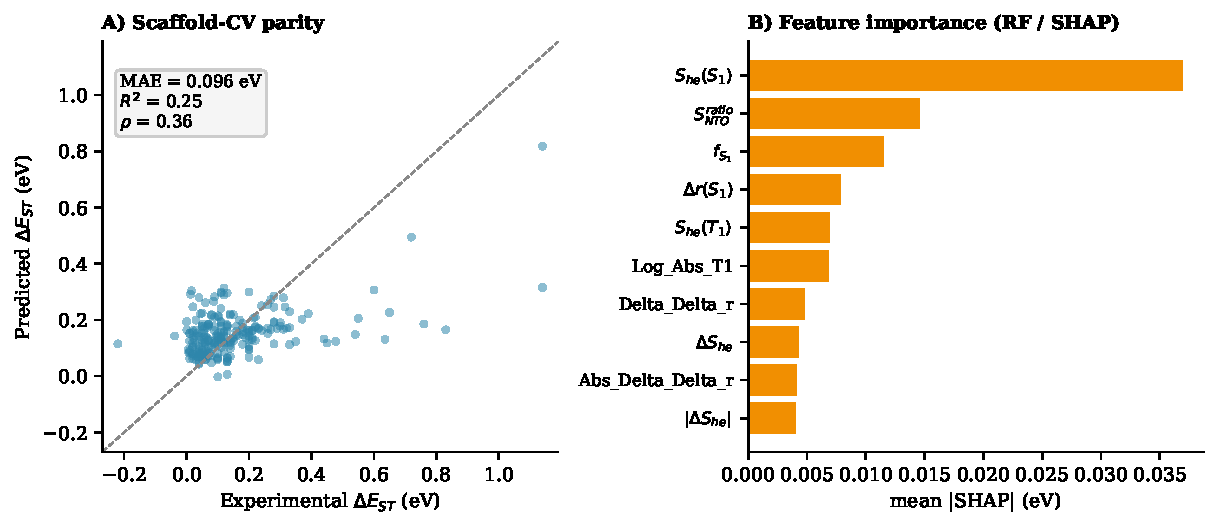
\includegraphics[width=0.95\textwidth]{figures/fig1_model_performance.pdf}
  \caption{Structure-based prediction of experimental $\Delta E_\text{ST}$.
    (A)~Scaffold cross-validated parity for the random forest on NTO
    spatial descriptors (\num{231} molecules, \num{212} Bemis--Murcko scaffolds):
    MAE = \qty{0.096}{\electronvolt}, $R^2 = 0.25$, Spearman $\rho = 0.36$. Models
    built from the 2D structure alone (Morgan, RDKit) perform equivalently
    (\cref{tab:feature_comparison}). The
    model regresses high-gap outliers toward the mean, the expected behaviour
    when the training distribution is dominated by low-gap emitters.
    (B)~SHAP importances: hole--electron overlap $S_\text{he}$, NTO overlap ratio,
    oscillator strength $f_{S_1}$ and charge-transfer distance $\Delta r$ dominate,
    consistent with exchange-integral physics.}
  \label{fig:model_performance}
\end{figure}

We assembled \num{231} donor--acceptor molecules for which an experimental
$\Delta E_\text{ST}$ could be matched to a structure, and evaluated random-forest
regressors under Bemis--Murcko scaffold cross-validation (\num{212} distinct
scaffolds), so that no scaffold appears in both training and test.
Because \qty{92.9}{\percent} of scaffolds are singletons, scaffold and random splits
produce numerically similar folds (test--train nearest-neighbour Tanimoto differs by
only \num{0.022}). The scaffold split guarantees zero shared scaffolds per fold
(versus \numrange{3}{8} under a random split) but task difficulty barely changes;
the harder test of transfer is the source-paper split reported below.
That the model learns real signal rather than
scaffold-group structure is confirmed by a label-permutation test: the true
scaffold-CV MAE (\qty{0.096}{\electronvolt}) lies far below the null from
\num{1000} target shuffles (mean \qty{0.120}{\electronvolt}, $p = 0.001$;
\cref{SI-tab:scaffold}).
The headline accuracy is also stable across validation schemes: replacing the singleton
scaffolds with genuine multi-molecule Butina clusters (down to \num{70} groups, largest
\num{38} molecules) leaves the MAE at \qtyrange{0.099}{0.104}{\electronvolt}, between
scaffold-CV (\qty{0.096}{\electronvolt}) and random-CV (\qty{0.106}{\electronvolt})
(\cref{SI-tab:clustercv}).
The three feature sets perform within \qty{0.009}{\electronvolt} of one another
(\cref{tab:feature_comparison}); for the fingerprint and excited-state models, which we
compare head to head below, that closeness is backed by a paired bound of
\qty{0.017}{\electronvolt}. Two are computed from the 2D structure alone, with
no quantum chemistry: Morgan fingerprints (MAE = \qty{0.091}{\electronvolt}) and
RDKit physicochemical descriptors (\qty{0.100}{\electronvolt}). The third, NTO spatial
descriptors, is derived from a semi-empirical sTDA excited-state calculation but
excludes the $S_1$/$T_1$ energy scalars; it reaches MAE = \qty{0.096}{\electronvolt}
(\qty{95}{\percent} CI \numrange{0.082}{0.109}), $R^2 = 0.25$ (CI
\numrange{0.03}{0.45}), Spearman $\rho = 0.36$.
That the structure-only sets match the NTO set is the central methodological point:
the excited-state calculation buys no accuracy, and adding back the $S_1$/$T_1$ energies
does not help either (\cref{tab:feature_comparison}).
The natural comparator is the mean-value baseline (MAE = \qty{0.107}{\electronvolt}),
over which every model improves by only about \qty{10}{\percent}; the large apparent
gain over the raw sTDA gap (\qty{0.25}{\electronvolt}) reflects that the semi-empirical
gap is badly biased, not that the model is accurate.
The $R^2$ confidence intervals are wide and, for the structure-only sets, include
negative values (RDKit \numrange{-0.11}{0.51}; Morgan \numrange{-0.19}{0.53}): at
\qty{95}{\percent} confidence we cannot exclude that these models are no better than
predicting the mean. The signal is real but weak.

A higher level of theory does not change this picture. A range-separated TD-DFT
gap (wB97X-D4/def2-SVP, Tamm--Dancoff, \num{609} core-hours) overestimates the
measured gap by a systematic \qty{0.65}{\electronvolt} and, used directly, is the
least accurate predictor in \cref{tab:feature_comparison} (MAE
\qty{0.654}{\electronvolt}, $R^2 = -16.3$). Its correlation with experiment is
higher than the semi-empirical gap's (Pearson $r$ from \num{0.32} to \num{0.43}),
and an in-fold linear calibration that removes the offset brings it to MAE
\qty{0.099}{\electronvolt}---level with the mean-value baseline, still short of
the structure-only forest. Added as a single feature it lowers the Morgan model
from \num{0.091} to \qty{0.087}{\electronvolt} (paired \qty{95}{\percent} CI
\numrange{0.0004}{0.0071}, Wilcoxon $p = 0.016$): a real but \qty{4}{\percent}
effect for \num{609} core-hours (\cref{SI-tab:tddft_headtohead}). The
excited-state step, semi-empirical or TD-DFT, does not move the structure-only
result.

Holding out whole source papers rather than scaffolds is a stricter test: it
removes a synthetic series and a laboratory's shared measurement practice together --- a
proxy for protocol, since the corpus records no measurement conditions per value. Under a
DOI-grouped \texttt{GroupKFold} (\num{173} papers, \num{231} molecules) the
Morgan model reaches MAE \qty{0.102}{\electronvolt} ($R^2 = 0.18$), and its
paired advantage over the mean-value baseline falls to \qty{0.005}{\electronvolt}
with a \qty{95}{\percent} CI that crosses zero. On \emph{accuracy}, then, the model
does not demonstrably transfer to an unseen source laboratory; part of the
scaffold-CV signal is within-paper regularity.

Ranking behaves differently, and this is the one place the excited-state features
separate from the fingerprints. Across the same DOI folds the NTO model holds
Spearman $\rho = \num{0.35}$ while Morgan drops to \num{0.16}
(MAE \qty{0.099}{\electronvolt} against \qty{0.102}{\electronvolt}); the paired
difference $\Delta\rho = \num{0.19}$ has a \qty{95}{\percent} CI of
\numrange{0.04}{0.34} and excludes zero, though only just; the resampling is over
molecules rather than over the \num{173} source papers, so a group-level interval would
be wider, and this is a single comparison on a single split rather than a general
result. Since Spearman $\rho$ is the metric we
report as primary for triage (\cref{sec:methods}), the semi-empirical excited-state
step earns its cost for ordering candidates across laboratories even though it earns
nothing for the value of the gap. One observation bounds the pessimistic reading, with a caveat that must travel with it:
\qty{58}{\percent} of repeatedly-measured molecules have zero inter-report spread, and
on the \num{102}-molecule multi-report subset the model reaches the study's lowest MAE,
\qty{0.080}{\electronvolt}. That subset is also an easier target: a mean-value predictor
restricted to it scores \qty{0.089}{\electronvolt}, so the model's advantage there is
\qty{0.009}{\electronvolt} with a \qty{95}{\percent} CI spanning zero. The low absolute
error reflects the narrower spread of those labels more than any gain in prediction.

\begin{table}[htbp]
  \centering
  \caption{Prediction of experimental $\Delta E_\text{ST}$ under scaffold
    cross-validation (random forest, \num{231} molecules); $R^2$ with \qty{95}{\percent}
    bootstrap CI. The 2D-structure-only sets (no quantum chemistry) match the
    NTO set, which requires an sTDA excited-state run; none approaches the
    precision a quantitative photophysical method would require, and the
    structure-only $R^2$ intervals include zero. The range-separated TD-DFT
    reference gap (wB97X-D4/def2-SVP, Tamm--Dancoff; \num{609} core-hours) is
    listed raw, after an in-fold linear calibration, and as an added feature
    (\cref{SI-tab:tddft_headtohead}).}
  \label{tab:feature_comparison}
  \begin{tabular}{lccc}
    \toprule
    Feature set & MAE (eV) & $R^2$ (95\% CI) & Spearman $\rho$ \\
    \midrule
    Morgan FP (2D structure only)   & 0.091 & 0.27 ($-0.19$, 0.53) & 0.31 \\
    RDKit desc.\ (2D structure only) & 0.100 & 0.31 ($-0.11$, 0.51) & 0.26 \\
    NTO spatial (needs sTDA)        & 0.096 & 0.25 (0.03, 0.45) & 0.36 \\
    Energies + NTO (reference)      & 0.097 & 0.24 & 0.34 \\
    \midrule
    Mean-value baseline             & 0.107 & 0.00 & --- \\
    Raw sTDA gap                    & 0.251 & $-2.22$ & 0.24 \\
    \midrule
    \multicolumn{4}{l}{\emph{Physics reference gaps (higher level of theory)}} \\
    Raw TD-DFT gap (wB97X-D4/def2-SVP) & 0.654 & $-16.3$ & 0.38 \\
    Calibrated TD-DFT gap (in-fold)    & 0.099 & 0.17 & 0.37 \\
    Morgan FP $+$ TD-DFT gap           & 0.087 & 0.31 & 0.37 \\
    \bottomrule
  \end{tabular}
\end{table}

For the NTO variant, SHAP (SHapley Additive exPlanations) analysis
(\cref{fig:model_performance}B) identifies
hole--electron overlap $S_\text{he}$, the NTO overlap ratio, oscillator strength
$f_{S_1}$ and the charge-transfer distance $\Delta r$ as the dominant
predictors---spatial quantities that encode the exchange integral governing
$\Delta E_\text{ST}$. This ranking is stable rather than an artefact of one fit:
across \num{200} bootstrap refits the leading descriptor $S_\text{he}(S_1)$ stays
in the top five \qty{99.5}{\percent} of the time, and on average \num{3.7} of the
five canonical descriptors recur (\cref{SI-tab:shapboot}). Restricting the attribution to
the reliable-prediction subset---the \num{152} molecules whose out-of-fold residual is
below \qty{0.10}{\electronvolt}---leaves $S_\text{he}(S_1)$ ranked first in
\qty{99.5}{\percent} of refits, so the leading attribution does not rest on the
poorly-predicted tail. An independent, model-agnostic permutation-importance analysis ranks the same
descriptor, $S_\text{he}(S_1)$, first, so the leading attribution is corroborated by
two methods (the lower-ranked tail is not; SI section~S6.3). Given the model's modest
ranking power, we read only the dominant attribution as a mechanistic hypothesis for
experimental test rather than a validated causal claim; the structure-only
fingerprint and descriptor models reach the same accuracy without any excited-state
calculation.

\subsection{Structural descriptors are sufficient: an informative null result}\label{subsec:nto_null}

Do quantum-mechanical features beat pure structural descriptors when the target is an
experimental property? For accuracy, no---and we can now put a bound on the word.
Paired on identical folds, the NTO model (MAE $= \qty{0.096}{\electronvolt}$) and the
Morgan model ($\qty{0.091}{\electronvolt}$) differ by
$\Delta\text{MAE} = \qty{-0.004}{\electronvolt}$ (\qty{95}{\percent} CI
\numrange{-0.017}{0.009}, Wilcoxon $p = 0.66$). The two feature sets are therefore
equivalent to within \qty{0.017}{\electronvolt}---an equivalence margin roughly a third
of the \qty{0.049}{\electronvolt} precision of the label itself, not merely a failure to
reject. Both beat the mean-value baseline by \qtyrange{10}{15}{\percent} MAE (paired CI
excludes zero), and the excited-state step adds nothing to that margin.

The equivalence is a statement about \emph{accuracy}, and it does not extend to
\emph{ranking} under protocol transfer. Under the source-paper split
(\cref{subsec:benchmark}) the NTO model retains Spearman $\rho = 0.35$ while the Morgan
model falls to \num{0.16}; the paired difference is
$\Delta\rho = \num{0.19}$ (\qty{95}{\percent} CI \numrange{0.04}{0.34}, excluding
zero). On the labelled benchmark the same asymmetry appears in triage: at the top
\qty{20}{\percent} the NTO model enriches low-gap emitters \num{1.6}-fold against
\num{1.4}-fold for Morgan. The excited-state calculation does not buy accuracy on the
gap; it buys ordering that survives a change of source laboratory, which is what a
triage filter is actually asked to do. Recent theoretical work by Salvi et al.~\cite{Salvi2025} on electronic correlation
effects explains why semi-empirical excited-state features may not outperform 2D features
against experimental gaps: at the semi-empirical level, the charge-transfer excitation
energies are not quantitatively accurate enough to provide additional discrimination
beyond what 2D topology already encodes.
The two representations differ in what they can be read for, though not in a way the
attribution totals establish on their own. The ten highest-attribution NTO descriptors
carry \qty{79}{\percent} of that model's SHAP weight against \qty{30}{\percent} for the
ten highest-attribution Morgan bits (\cref{SI-fig:shapcompare}); those totals are not
comparable, because ten descriptors are \qty{29}{\percent} of the \num{35}-dimensional
NTO set and ten bits are \qty{0.5}{\percent} of a \num{2048}-bit fingerprint, so the
concentration follows from dimensionality. What does not follow from dimensionality is
that the NTO features are \emph{named} donor--acceptor overlap and charge-transfer
quantities, whereas Morgan bits are anonymous hashed substructures. The case for the
physics-informed representation is interpretability of the variables themselves, not a
larger share of attribution.

\subsection{What limits achievable accuracy}\label{subsec:ceilings}

Accuracy near \qty{0.1}{\electronvolt} is limited by the data rather than by the model,
and the term that applies is the quality of the label.
Independent experimental reports for the same compound disagree
substantially: a single randomly chosen report sits \qty{0.072}{\electronvolt} from its
molecule's median (RMS with each molecule weighted equally), the disagreement exceeds the
model MAE for \qty{19.6}{\percent} of molecules, and the worst molecule reaches a standard
deviation of \qty{0.56}{\electronvolt}; the eight independent values for 4CzIPN alone span
\qtyrange{0.01}{0.48}{\electronvolt} (\cref{SI-tab:solvent}).
The quantity the model is regressed on, however, is the per-molecule \emph{median},
whose precision is better than any single report: the RMS standard error of that median
is \qty{0.049}{\electronvolt}, about half the model MAE. Label imprecision is therefore
a real term in the error budget but does not by itself account for it, and we do not
claim the forest sits at a noise floor.
A second, separate dispersion applies to computed references rather than to this
regression: the computed gap is functional-dependent. Across the
\num{7} molecules (gas and toluene) for which we ran both B3LYP/6-31G(d) and CAM-B3LYP/def2-TZVP,
$\Delta E_\text{ST}$ differs by a mean \qty{0.30}{\electronvolt} (up to
\qty{0.58}{\electronvolt}) and changes
relative magnitude (\cref{SI-tab:dft_benchmark}); a higher-tier benchmark across
six range-separated functionals on \num{27} emitters~\cite{Froitzheim2024} shows the same
effect at finer resolution: a median inter-functional spread of \qty{0.05}{\electronvolt}
on a quantity that approximates \emph{half} the gap, hence roughly
\qty{0.1}{\electronvolt} on \deltaest\ itself. Any claim of sub-\qty{0.1}{\electronvolt}
accuracy against such a reference is not physically meaningful. This second effect bounds
what a \emph{computed} gap can mean; it does not bound a model regressed on measured
labels, and we do not add the two into a single floor. Only the label term applies
directly to the present task. What both establish is that richer feature sets and
alternative regressors are not the missing ingredient. We tested both directly. No higher-capacity learner beats the
random forest under the same scaffold CV. Histogram gradient boosting reaches
\qty{0.105}{\electronvolt}, an MLP \qty{0.169}{\electronvolt} and an RBF SVR
\qty{0.120}{\electronvolt} (\cref{SI-tab:capacity}); a second comparison over a
differently configured set of learners places plain gradient boosting at
\qty{0.098}{\electronvolt}, within \qty{0.002}{\electronvolt} of the forest and so
inside the equivalence margin established above
(\texttt{code/a007\_leakage\_and\_nested\_cv.py}; \cref{SI-tab:capacity} lists the
histogram-boosting configuration). Added
capacity therefore does not help, though we would not claim the forest is uniquely
suited; and the negative lower $R^2$ bound is not a
fingerprint-width artefact, since \num{512}-, \num{1024}- and \num{2048}-bit Morgan models
share it (\cref{SI-tab:capacity}).

Stratifying by label quality does not isolate a label effect, and the attempt is
instructive. Restricting to molecules that carry replicates, the model reaches MAE
\qty{0.074}{\electronvolt} on the \num{79} whose reports agree to
$\le\qty{0.05}{\electronvolt}$, \qty{0.106}{\electronvolt} on the \num{23} whose
reports do not, and \qty{0.107}{\electronvolt} on the \num{129} for which label
precision cannot be measured. That ordering is not evidence about labels: a constant
predictor fitted within each stratum reproduces it almost exactly
(\qty{0.074}{}, \qty{0.107}{} and \qty{0.110}{\electronvolt}), because the strata
differ in the dispersion of the target itself (standard deviation \qty{0.10}{},
\qty{0.15}{} and \qty{0.20}{\electronvolt}). Within any one stratum the model carries
no advantage over a constant. We therefore report no stratified evidence for a label
ceiling; the quantitative statement that survives is the precision of the median target,
\qty{0.049}{\electronvolt} (above).

A related question is whether \emph{uncontrolled measurement conditions}, rather than
label imprecision as such, set the limit. The corpus records no solvent, host or
temperature for individual values, so a strictly condition-controlled subset cannot be
built; the closest proxy is the source paper, since molecules whose values all come from
one publication were measured under one laboratory's conditions. Splitting the benchmark on that
(\num{218} single-source against \num{13} multi-source molecules) and scoring the random
forest on the same scaffold cross-validation folds, the model's advantage
over a constant baseline predictor fitted within each group is \qty{0.0071}{} and
\qty{0.0024}{\electronvolt} respectively, a difference of \qty{0.005}{\electronvolt}
with a \qty{95}{\percent} CI of \numrange{-0.014}{0.035} that includes zero. The raw
errors run the other way (\qty{0.058}{} against \qty{0.093}{\electronvolt}) but the
multi-source group's target dispersion is half as large and its own constant predictor
scores \qty{0.061}{\electronvolt}, so that ordering is again dispersion rather than
label quality. With only \num{13} molecules drawing on more than one paper the test
constrains the effect rather than excluding it; we find no evidence that mixed conditions
drive the error, and do not claim conditions are irrelevant.

The corpus size is not the limit either. Featurising \num{497} additional
experimental emitters through the same pipeline (a \num{728}-molecule set) raises
the MAE from \qty{0.098}{} to \qty{0.124}{\electronvolt}, drives $R^2$ from
\num{0.18} to $-0.01$, and roughly halves the rank correlation (Spearman $\rho$
from \num{0.34} to \num{0.16}); the replicate-measured subset
($n = \num{465}$) recovers only about half of the loss (\cref{SI-tab:expansion}).
Tripling the training data makes the prediction worse. The added molecules are resolved
through a different structure pipeline, so wider chemical space and lower label quality are
confounded and this test cannot separate them; what it does rule out is the reading that
the corpus is simply too small.

A separate concern is the descriptor side: the NTO features are computed at the
\emph{vertical} (ground-state) geometry, whereas the measured gap reflects relaxed
excited states. We bounded this approximation by recomputing \deltaest\ adiabatically
for \num{14} representative emitters in gas and toluene at CAM-B3LYP/def2-TZVP with
excited-state optimisation (\cref{SI-tab:adiabatic}). Relative to these adiabatic
references the vertical gap carries a mean absolute deviation of
\qty{0.195}{\electronvolt}, which exceeds the model's own error. The deviation is
dominated by an additive offset rather than by reordering---a linear fit gives slope
\num{1.00} and intercept \qty{0.07}{\electronvolt} ($R^2 = 0.70$, Spearman
$\rho = 0.71$)---so relaxation shifts the scale more than it scrambles the ranking the
triage relies on. The residual is not negligible, however: the RMS deviation is
\qty{0.245}{\electronvolt} and the worst molecule departs by \qty{0.548}{\electronvolt},
with sign changes between compounds, and \num{14} molecules cannot settle how much of
that is systematic. We take the vertical descriptors as an acceptable ranking input on
this evidence, not as a validated approximation to the adiabatic gap.

\subsection{Candidate prioritisation as a triage filter}\label{subsec:candidates}

The model's practical value is as a coarse triage filter: it eliminates the bottom
tier of candidates rather than ordering the viable subset. We quantify this directly. Taking emitters with experimental
$\Delta E_\text{ST}\le\qty{0.10}{\electronvolt}$ as the targets (\qty{49}{\percent}
of the set), the structure-only model's top-ranked candidates are enriched in
targets relative to random selection by \numrange{1.2}{1.4}$\times$
(precision rising from the \qty{49}{\percent} base rate to \qty{60}{\percent} at
the top \num{10}--\num{20} and \qty{68}{\percent} at the top \num{50}).
Note that $\Delta E_\text{ST}$ is a necessary but not sufficient condition for TADF
efficiency; emission wavelength matching is a subsequent, independent design step
not addressed by this model.
The filter therefore works, but weakly: it is a coarse
first pass that modestly concentrates good emitters, not a selector.
Among well-characterised emitters, DMAC-DPS
(experimental $\Delta E_\text{ST}\approx\qty{0.09}{\electronvolt}$) and PXZ-NAI are
examples of low-gap emitters the filter retains.
Application to a specific lighting niche---horticultural or human-centric---is a
\emph{separate, downstream} step: it requires matching the emission wavelength and
oscillator strength, neither of which this scalar $\Delta E_\text{ST}$ model predicts.
We therefore make no spectral-matching or device-level claim (reverse intersystem
crossing rates and external quantum efficiencies depend on quantities this model does
not resolve, and our earlier device estimates did not survive scrutiny,
\cref{subsec:limitations}).

\subsection{A substructure-filtered extended chemical space}\label{subsec:library}

To indicate the chemical space such triage would operate over, we screened PubChem for
structures carrying both a donor and an acceptor motif, retaining \num{22194}
(\cref{sec:library_expansion}; molecular weights \qtyrange{172}{899}{\dalton},
\numrange{2}{12} aromatic rings; property distributions in
\cref{SI-fig:library_analysis}). Every member passes the donor--acceptor pattern test,
but the set carries the composition of the source database rather than of a designed
emitter series, and its matches lean on the weaker motifs; it indicates scale, not a
curated design space. We do not deposit a
ranked candidate list. On the filtered set the split-conformal
\qty{90}{\percent} prediction interval spans \qty{0.36}{\electronvolt} (mean
half-width \qty{0.18}{\electronvolt}), about \num{7.6} times the predicted gap, and for
every one of the \num{100} lowest-predicted molecules the interval's lower bound
falls below zero. At this accuracy conformal prediction refuses selection at the
single-molecule level; the filtered set only indicates the scale of the space that the
labelled-data triage would operate over. The heuristic score of
\cref{eq:tadf_score} remains a planning aid, not a calibrated predictor, and the
retained molecules are not quantum-validated.

\paragraph{Quantifying triage utility.}
On held-out labelled molecules the structure-only model enriches the low-gap
class by \numrange{1.2}{1.4}$\times$ over random selection: against the
\qty{49}{\percent} base rate
($\Delta E_\text{ST} \le \qty{0.10}{\electronvolt}$), top-ranked precision rises
to \qty{60}{\percent} at the top \numrange{10}{20} candidates and
\qty{68}{\percent} at the top \num{50}. The full enrichment curve
(\cref{fig:enrichment}) peaks near \num{1.37}$\times$ at the top
\numrange{5}{20}\% and does not improve at more aggressive cuts; a split-conformal
calibration lets a laboratory fix an operating point at a stated confidence. This
is a statement about the labelled benchmark: the model supports \emph{triage},
not selection, and the interval widths of \cref{subsec:library} rule out
projecting a hit rate onto the unvalidated filtered library.

\begin{figure}[htbp]
  \centering
  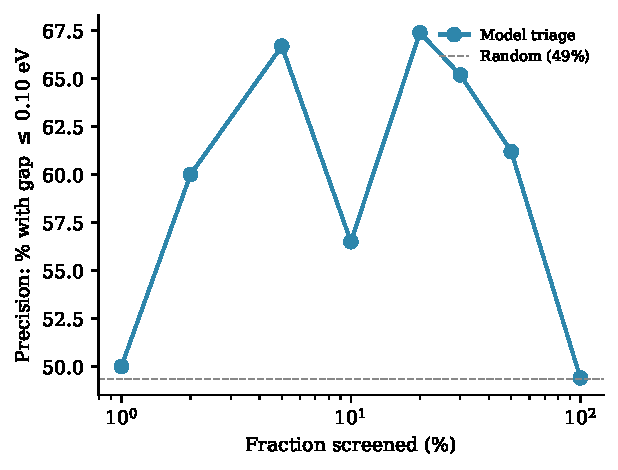
\includegraphics[width=0.7\textwidth]{figures/enrichment_curve.pdf}
  \caption{Triage precision versus fraction of the benchmark screened (log $x$).
    Dashed line: the \qty{49}{\percent} random base rate. Enrichment is real but
    bounded at $\approx 1.3$--$1.4\times$; the top \num{1}\% is two molecules.}
  \label{fig:enrichment}
\end{figure}

\subsection{Comparison with existing ML approaches}\label{subsec:comparison}

Before comparing models, we contextualise the absolute errors against three
baselines computed on the out-of-fold scaffold-CV predictions
(\cref{tab:baselines}; \qty{95}{\percent} bootstrap CIs, \num{2000} resamples):
the mean-value predictor (predicting $\bar{y}$ for every molecule,
MAE $= \qty{0.107}{\electronvolt}$), the median-value predictor
(MAE $= \qty{0.098}{\electronvolt}$), and a random-permutation null (mean MAE
over \num{1000} label shuffles, \qty{0.120}{\electronvolt}, \qty{95}{\percent}
interval \numrange{0.113}{0.127}).
The median is a tougher baseline than the mean because the experimental gap
distribution is right-skewed toward low-gap emitters; the permutation null is
clearly worse than either constant predictor, confirming that the trained model
exploits a real feature--label association rather than a fold artefact.
Our best model (RF--Morgan, MAE $= \qty{0.091}{\electronvolt}$) improves on the
mean baseline by \qty{15}{\percent}; the headline NTO model
(MAE $= \qty{0.096}{\electronvolt}$) improves by \qty{10.6}{\percent}
(\qty{0.011}{\electronvolt}, \qty{95}{\percent} CI on the paired difference
\numrange{0.003}{0.022}, excluding zero). The model edges even the skewed-median
baseline (\qty{0.098}{\electronvolt}).
This gain appears modest, and it should be read against the precision of the target:
across the \num{102} multi-report molecules a single report deviates from the median by
\qty{0.072}{\electronvolt} on average (RMS), the worst molecule reaching a standard
deviation of \qty{0.56}{\electronvolt}, while the median actually regressed on carries
an RMS standard error of \qty{0.049}{\electronvolt}. An MAE of
\qty{0.096}{\electronvolt} is therefore about twice the precision of its own target ---
close enough that label quality is a material term, far enough that we do not describe
the model as sitting at a floor.
As shown above (\cref{subsec:nto_null}), the excited-state NTO descriptors offer no
accuracy advantage over the purely structural sets, consistent with label noise
dominating any feature advantage at the current scale.

\begin{table}[htbp]
  \centering
  \caption{Naive baselines versus the structure-based model on the same
    \num{231}-molecule out-of-fold scaffold-CV predictions. MAE in eV with
    \qty{95}{\percent} percentile-bootstrap CI (\num{2000} resamples); the
    permutation row is the mean and central \qty{95}{\percent} of \num{1000}
    label shuffles. The median outperforms the mean (right-skewed target); the
    permutation null is worse than both, so the model captures real signal.
    Values from \texttt{code/compute\_baselines.py}.}
  \label{tab:baselines}
  \begin{tabular}{lcc}
    \toprule
    Predictor & MAE (eV) & 95\% CI \\
    \midrule
    Mean predictor          & 0.107 & (0.092, 0.124) \\
    Median predictor        & 0.098 & (0.081, 0.118) \\
    Random-permutation null & 0.120 & (0.113, 0.127) \\
    \midrule
    NTO-RF (this work)      & \textbf{0.096} & (0.082, 0.109) \\
    \bottomrule
  \end{tabular}
\end{table}

Prior ML for TADF gaps is best read by the \emph{reference} it predicts, not by
the headline error alone (\cref{tab:prior_ml}). The low MAEs in the literature are
all against \emph{computed} targets: G\'omez-Bombarelli et
al.~\cite{Gomez-Bombarelli2016} trained a neural network to reproduce a TD-DFT gap
inside a $>$\num{e6}-molecule screen, Thapa et al.~\cite{Thapa2025} screened a
large virtual library against semi-empirically computed gaps, and Barneschi et al.~\cite{Barneschi2024}
reach \qty{0.02}{\electronvolt} with a 3D message-passing network---but against
ADC(2) values, and for inverted-gap molecules rather than donor--acceptor TADF.
Predicting the \emph{experimental} gap is the harder task this paper addresses:
Nigam et al.~\cite{Nigam2024} found direct regression of the measured gap so
unreliable that they fell back to a good/bad classifier. Our
\qty{0.096}{\electronvolt}, under scaffold cross-validation and with label and
reference noise accounted for, shows that cheap structural features nonetheless
track the experimental gap to within $\approx\qty{0.1}{\electronvolt}$, about twice the
precision of the target itself. The contribution is not a record accuracy but a calibrated,
reproducible measure of how far cheap structural features reach, and a bounded
demonstration that the excited-state step buys no accuracy on that task---while
still buying rank order that transfers across source laboratories
(\cref{subsec:benchmark}).

\begin{table*}[htbp]
  \centering
  \caption{Machine-learning prediction of TADF singlet--triplet gaps, ordered by
    reference type. Low MAEs are obtained only against \emph{computed} gaps;
    against the \emph{experimental} gap, errors are substantially larger and
    direct regression is sometimes abandoned. Only values reported in the
    cited sources are tabulated.}
  \label{tab:prior_ml}
  \small
  \begin{tabular}{lllll}
    \toprule
    Study & Model (features) & Set ($N$) & Reference & MAE (eV) \\
    \midrule
    G\'omez-Bombarelli 2016~\cite{Gomez-Bombarelli2016} & NN surrogate & $>$\num{e6} screened & TD-DFT (computed) & reproduces TD-DFT$^{a}$ \\
    Barneschi 2024~\cite{Barneschi2024} & 3D message-passing GNN & INVEST set & ADC(2) (computed) & 0.02$^{b}$ \\
    Nigam 2024~\cite{Nigam2024} & DNN classifier (Morgan FP) & GA-evolved & $\omega$B2PLYP$'$ (computed) & regression poor$^{c}$ \\
    \textbf{This work} & RF (NTO, structure) & 231 & experimental & \textbf{0.096} \\
    \bottomrule
  \end{tabular}

  \vspace{2pt}
  {\footnotesize\raggedright
   $^{a}$~Predicts the TD-DFT gap; no experimental-reference regression MAE reported.
   $^{b}$~Inverted-gap (Hund's-rule-violating) molecules, not donor--acceptor TADF.
   $^{c}$~Direct gap regression reported as poor; the deployed model is a good/bad
   classifier (\qtyrange{89}{98}{\percent} accuracy).\par}
\end{table*}

\subsection{Limitations}\label{subsec:limitations}

This study is bounded in several ways.
(1)~The experimental corpus is heterogeneous (mixed solvents and methods,
\qty{0.072}{\electronvolt} RMS inter-report scatter); a single-source,
solvent-controlled dataset would be required to push below the present ceiling.
(2)~The model predicts a consensus gap, not solvatochromic or
conformer-dependent values.
(3)~We make no quantitative device claims.
Molecule-independent estimates for spin–orbit coupling, $k_\text{RISC}$, and external quantum efficiency, derived from literature medians, were deliberately 
excluded from this analysis.
% An earlier version of this work included
% molecule-independent estimates for spin--orbit coupling, $k_\text{RISC}$, and
% external quantum efficiency derived from literature medians. Following internal peer
% review, these estimates were removed because the inter-molecular variance in these
% quantities exceeds the precision of a scalar estimate by an order of magnitude. We
% view this correction as an illustration of the iterative rigour appropriate to an
% honest benchmark study: a median is not a molecule-specific prediction, and
% reporting it as such would be misleading.
(4)~Ranking power is moderate ($\rho = 0.36$), so the model supports triage, not
final candidate selection.
(5)~The target is a single scalar, $\Delta E_\text{ST}(S_1\text{--}T_1)$. A small
$S_1$--$T_1$ gap is necessary but not sufficient for efficient delayed fluorescence:
the splitting of the triplet manifold ($T_1$--$T_2$) also governs reverse intersystem
crossing.\cite{Keruckiene2024} To gauge this we extracted $T_1$ and $T_2$ from the
CAM-B3LYP TD-DFT calculations for \num{14} emitters (\cref{SI-tab:manifold}): the
$T_1$--$T_2$ gap ranges \qtyrange{0.02}{1.50}{\electronvolt} and varies widely
\emph{among molecules with near-equal $\Delta E_\text{ST}$}, so a scalar-gap triage
cannot rank them on RISC propensity. The semi-empirical step is redundant for the
$S_1$--$T_1$ gap (\cref{subsec:nto_null}) and does at least yield a triplet-manifold
quantity that 2D structure does not, but we cannot show that quantity is reliable.
Extending the sTDA extraction to all \num{231} emitters, \qty{74}{\percent} carry a
$T_1$--$T_2$ gap below \qty{0.3}{\electronvolt}; that classification should be treated
as indicative only, since the deviation of the sTDA manifold from the CAM-B3LYP reference
(\qty{0.24}{\electronvolt}, below) is comparable to the \qty{0.3}{\electronvolt}
threshold being applied.
We read this full-corpus manifold only qualitatively: benchmarked against the
\num{14}-molecule CAM-B3LYP reference (six molecules overlapping), the sTDA $T_1$--$T_2$
gap carries a mean absolute deviation of \qty{0.24}{\electronvolt} and a rank
correlation that is not resolved at this sample size (Spearman $\rho = 0.43$,
$p = 0.40$, $n = 6$): the two methods agree on neither magnitude nor rank at a useful
level, so quantitative ranking on RISC propensity requires the higher-level calculation
(\cref{SI-tab:manifold}). Emitters with an \emph{inverted} gap ($\Delta E_\text{ST}<0$), which violate
Hund's rule through double-excitation character,\cite{Veglianti2025} are out of
scope, and the model fails on them exactly as its construction requires. A literature
screen flags \num{5} corpus compounds for which at least one report gives an inverted
gap; for two of these the consensus median we train on is itself negative
(HAP-3MF, \qty{-0.22}{\electronvolt}; TPA-NZP, \qty{-0.038}{\electronvolt}), and these
are the only \num{2} negative labels among the \num{231}. The random forest---built on
GFN2-xTB features that enforce Aufbau ordering---returns a positive gap for all five, so
it carries the wrong sign for both molecules whose own training label is negative. The failure is representational rather than incidental. A regression forest can in
principle return a negative value, since its output is an average over training labels and
two of ours are negative; what it lacks is any feature that separates an inverted-gap
molecule from a conventional one, because the sTDA descriptors are computed under Aufbau
ordering and the structure-only descriptors carry no excited-state information at all.
Predicting this class would require descriptors that encode double-excitation character,
not more data (\cref{SI-fig:istdist}). Screening this
class would require ROKS- or EOM-CCSD-level descriptors.\cite{Salvi2025}
(6)~The semi-empirical descriptors are computed at ground-state vertical geometries and
therefore carry no information about excited-state structural relaxation, and none about
spin--orbit coupling. Both matter physically for delayed fluorescence, and the omission is
a plausible part of why the NTO features do not outperform 2D fingerprints: a vertical
descriptor cannot represent the charge-transfer relaxation that separates two molecules with
similar ground-state topology. Our \num{14}-molecule adiabatic comparison bounds the size of
the vertical approximation (mean absolute deviation \qty{0.195}{\electronvolt}, RMS
\qty{0.245}{\electronvolt}) but cannot remove it, and excited-state optimisation for the
full corpus was outside the compute budget. Descriptors built on relaxed excited-state
geometries are the natural next test of whether the equivalence reported here survives.

(7)~Under a source-paper (DOI-grouped) split the model's advantage over a
mean-value predictor is not statistically resolved (\cref{subsec:benchmark});
demonstrated transfer is to new scaffolds measured under represented protocols,
not to new measurement laboratories.
Future work targets a curated experimental benchmark and uncertainty-aware models
that report calibrated confidence alongside each prediction.
